%%%%%%%%%%%%%%%%%%%%%%%%%%%%%%%%%%%%%%%%%
% Jacobs Landscape Poster
% LaTeX Template
% Version 1.0 (29/03/13)
%
% Created by:
% Computational Physics and Biophysics Group, Jacobs University
% https://teamwork.jacobs-university.de:8443/confluence/display/CoPandBiG/LaTeX+Poster
% 
% Further modified by:
% Nathaniel Johnston (nathaniel@njohnston.ca)
%
% This template has been downloaded from:
% http://www.LaTeXTemplates.com
%
% License:
% CC BY-NC-SA 3.0 (http://creativecommons.org/licenses/by-nc-sa/3.0/)
%
%%%%%%%%%%%%%%%%%%%%%%%%%%%%%%%%%%%%%%%%%

%----------------------------------------------------------------------------------------
%	PACKAGES AND OTHER DOCUMENT CONFIGURATIONS
%----------------------------------------------------------------------------------------

\documentclass[final]{beamer}
\usepackage[official]{eurosym}


\usepackage[scale=1.24]{beamerposter} % Use the beamerposter package for laying out the poster

\usetheme{confposter} % Use the confposter theme supplied with this template

\setbeamercolor{block title}{fg=ngreen,bg=white} % Colors of the block titles
\setbeamercolor{block body}{fg=black,bg=white} % Colors of the body of blocks
\setbeamercolor{block alerted title}{fg=white,bg=dblue!70} % Colors of the highlighted block titles
\setbeamercolor{block alerted body}{fg=black,bg=dblue!10} % Colors of the body of highlighted blocks
% Many more colors are available for use in beamerthemeconfposter.sty

%-----------------------------------------------------------
% Define the column widths and overall poster size
% To set effective sepwid, onecolwid and twocolwid values, first choose how many columns you want and how much separation you want between columns
% In this template, the separation width chosen is 0.024 of the paper width and a 4-column layout
% onecolwid should therefore be (1-(# of columns+1)*sepwid)/# of columns e.g. (1-(4+1)*0.024)/4 = 0.22
% Set twocolwid to be (2*onecolwid)+sepwid = 0.464
% Set threecolwid to be (3*onecolwid)+2*sepwid = 0.708
\definecolor{dorado}{RGB}{255,204,102}
\newlength{\sepwid}
\newlength{\onecolwid}
\newlength{\twocolwid}
\newlength{\threecolwid}
\setlength{\paperwidth}{48in} % A0 width: 46.8in
\setlength{\paperheight}{36in} % A0 height: 33.1in
\setlength{\sepwid}{0.024\paperwidth} % Separation width (white space) between columns
\setlength{\onecolwid}{0.22\paperwidth} % Width of one column
\setlength{\twocolwid}{0.464\paperwidth} % Width of two columns
\setlength{\threecolwid}{0.708\paperwidth} % Width of three columns
\setlength{\topmargin}{-0.5in} % Reduce the top margin size
%-----------------------------------------------------------

\usepackage{graphicx}  % Required for including images

\usepackage{booktabs} % Top and bottom rules for tables

%----------------------------------------------------------------------------------------
%	TITLE SECTION 
%----------------------------------------------------------------------------------------

\title{Rate My Apartments 2015} % Poster title

\author{CMPT 470, Group 7} % Author(s)

\institute{June 1 - Present } % Institution(s)

%----------------------------------------------------------------------------------------

\begin{document}

\addtobeamertemplate{block end}{}{\vspace*{2ex}} % White space under blocks
\addtobeamertemplate{block alerted end}{}{\vspace*{2ex}} % White space under highlighted (alert) blocks

\setlength{\belowcaptionskip}{2ex} % White space under figures
\setlength\belowdisplayshortskip{2ex} % White space under equations

\begin{frame}[t] % The whole poster is enclosed in one beamer frame

\begin{columns}[t] % The whole poster consists of three major columns, the second of which is split into two columns twice - the [t] option aligns each column's content to the top

\begin{column}{\sepwid}\end{column} % Empty spacer column

\begin{column}{\onecolwid} % The first column




%----------------------------------------------------------------------------------------
%	INTRODUCTION
%----------------------------------------------------------------------------------------

\begin{block}{Why ???}

\textbf{Why do we need this web application}\newline
- In 2011, there were 891,310 households in Metro Vancouver; 65 percent were owners and 35 percent were renters\newline
- According to the statistics, a significant amount of the population needs an accurate, objective, and unbiased information when renting a property\newline
- Currently, most potential tenants get information via vancouver.craigslist.ca, kijiji.ca, rentbc.com, and renthello.com \newline
- The main problem of the information from currently used websites is that the information is solely provided by owners: which can be inaccurate, subjective, and biased \newline\newline
\textbf{Rating} \newline
- Rate each Apt and write comments\newline
- Star Rating: Click on stars to give a score for each rating category\newline
- Provides avg score for each category for each Apt\newline

\end{block}


%
%--------------------------------------
%
\begin{block}{So What ???}
- We've come up with a web application to solve this problem\newline
- With our application you can easily find your home that best suits your needs\newline

\end{block}
\begin{block}{How ???}
- We have a ranking system that will allow potential tenants to see which Apts are HOT!\newline
- How does this ranking system work?\newline
- Based on other tenants' ratings on all attributes, our system will provide the overall ranking of the Apts.\newline\newline

\end{block}

%----------------------------------------------------------------------------------------

\end{column} % End of the first column

\begin{column}{\sepwid}\end{column} % Empty spacer column

\begin{column}{\twocolwid} % Begin a column which is two columns wide (column 2)

\begin{columns}[t,totalwidth=\twocolwid] % Split up the two columns wide column

\begin{column}{\onecolwid} % The first column within column 2 (column 2.1)

%----------------------------------------------------------------------------------------
%	Our work
%----------------------------------------------------------------------------------------


%----------------------------------------------------------------------------------------

\end{column} % End of column 2.1

\begin{column}{\onecolwid} % The second column within column 2 (column 2.2)

%----------------------------------------------------------------------------------------
%	How does it work
%----------------------------------------------------------------------------------------


%----------------------------------------------------------------------------------------

\end{column} % End of column 2.2

\end{columns} % End of the split of column 2 - any content after this will now take up 2 columns width

%----------------------------------------------------------------------------------------
%	IMPORTANT RESULT
%----------------------------------------------------------------------------------------

\begin{alertblock}{Interesting features}

\begin{itemize}
\item User Authentication: \newline- (Super) Admin has super powers. They can perform anything \newline - Regular users can rate/comment and vote. They can manipulate only what they create.\newline  - Guests can only view
\item Google Authentication: Users can sign up using their Google accounts
\item Search:\newline- Simple Search allows users to search by Apt name and address \newline- Advanced Search allows users to refine their preferences for recommendations
\item Auto-complete: Don't remember the full name of the Apt? Don't worry. Two letters will suffice
\item Contact Us: Have a question? Just fill out a form and we will get back to you ASAP. We will send you a confirmation email regarding your questions
\item Map: Don't know where the Apt is? Let us show you where the Apt is located on a Map

\end{itemize}
\end{alertblock} 

%----------------------------------------------------------------------------------------

\begin{columns}[t,totalwidth=\twocolwid] % Split up the two columns wide column again

\begin{column}{\onecolwid} % The first column within column 2 (column 2.1)


\begin{figure}
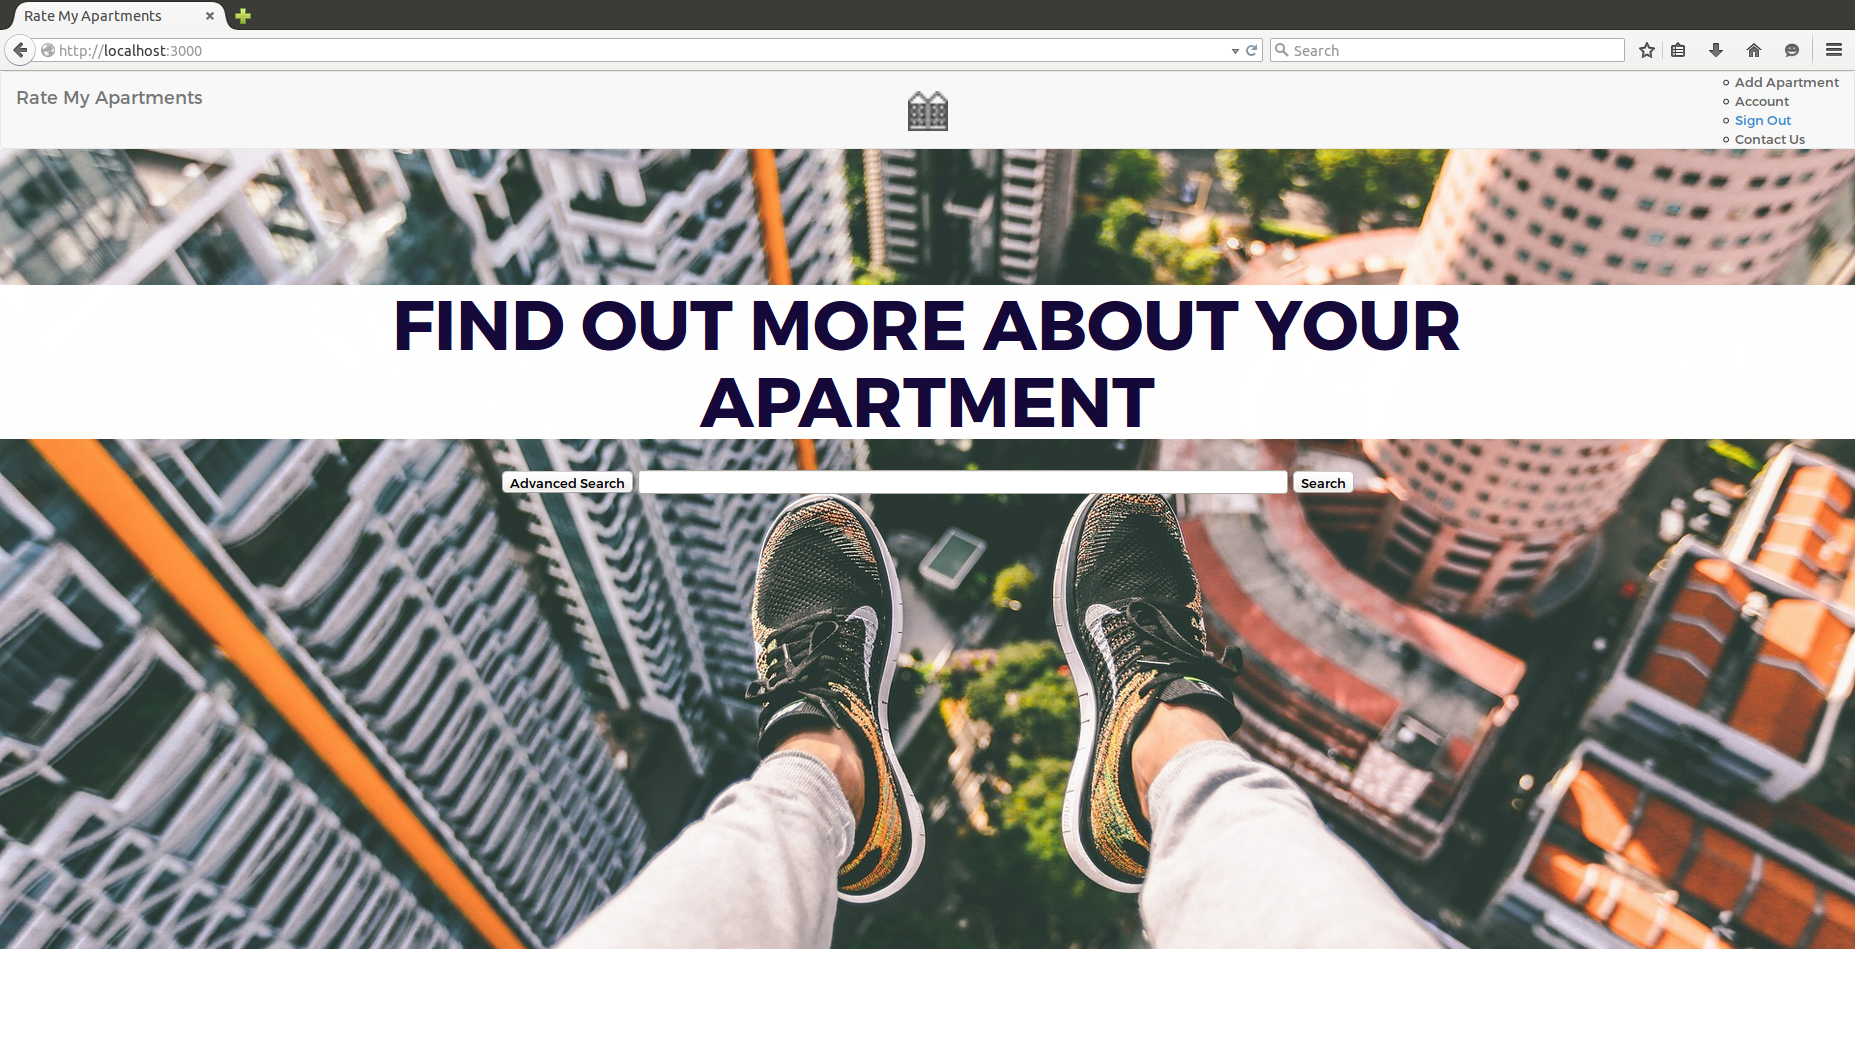
\includegraphics[height=0.5\linewidth]{mainpage.png}
\caption{Main Page}
\end{figure}

\begin{figure}
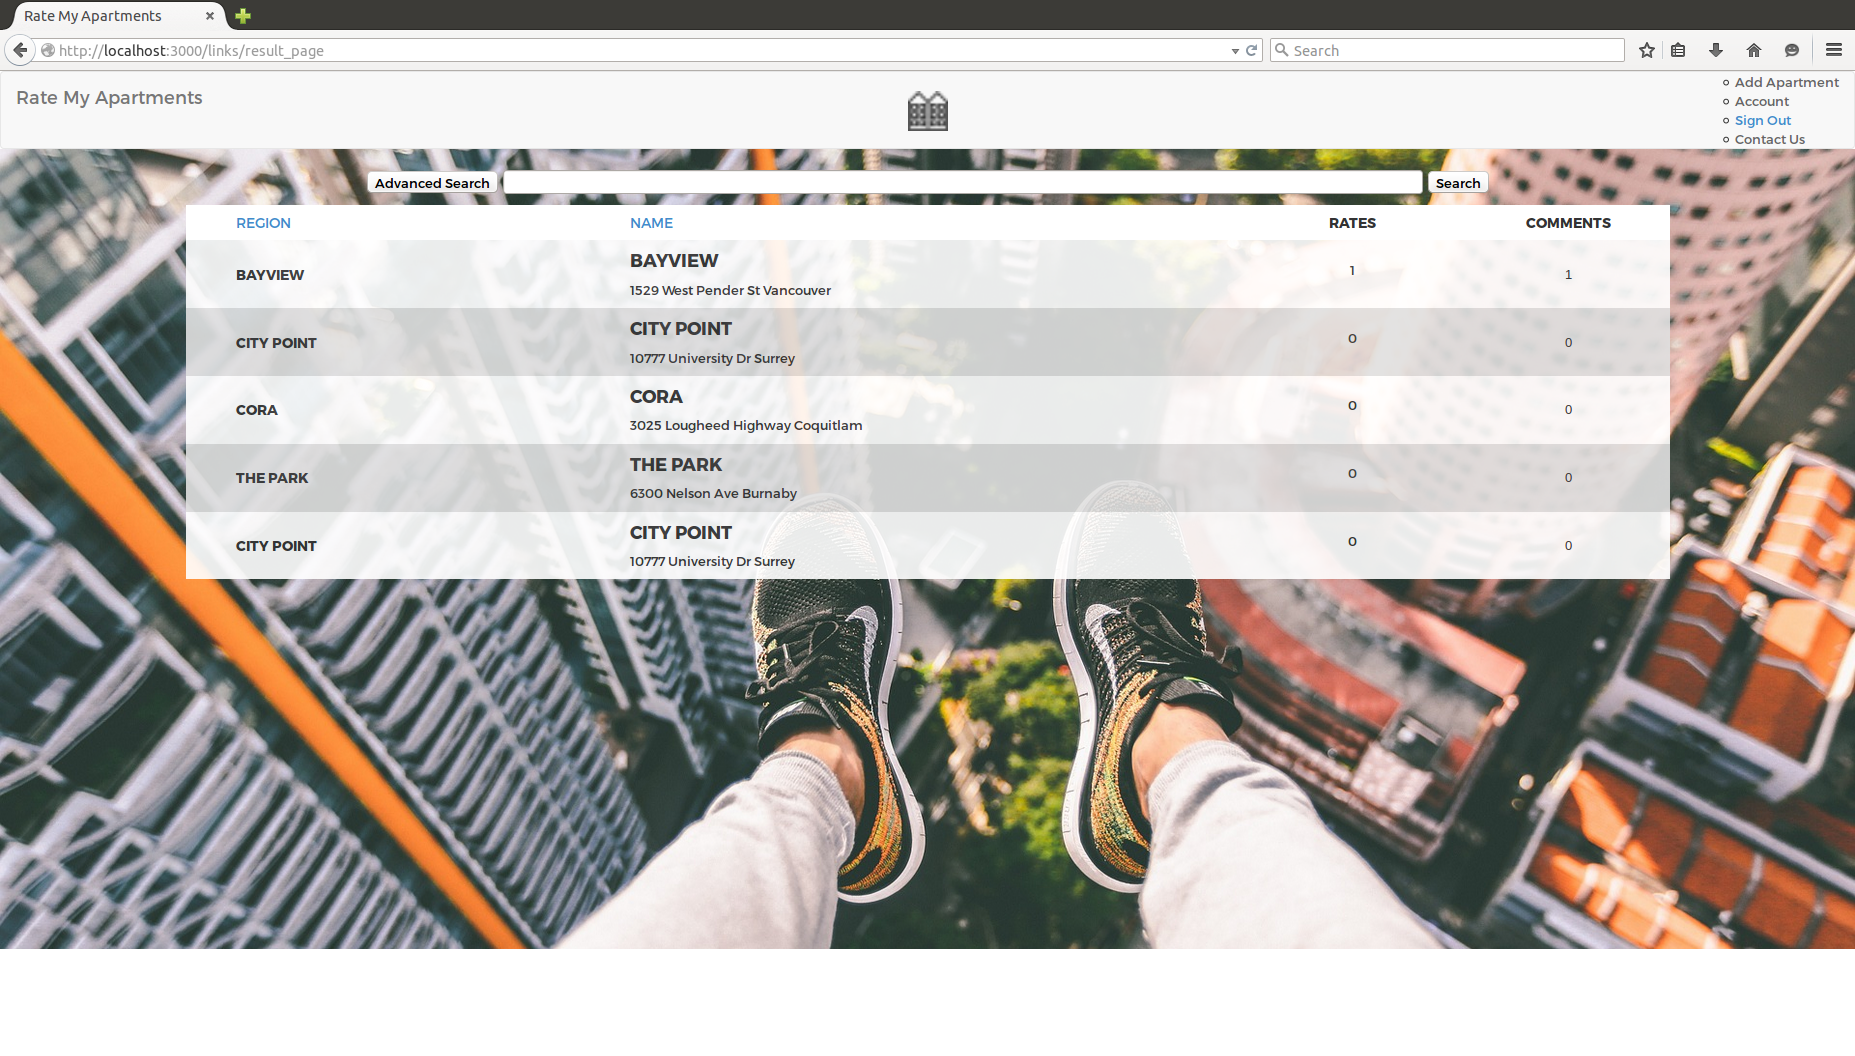
\includegraphics[height=0.5\linewidth]{table.png}
\caption{Table Page}
\end{figure}


\end{column} % End of column 2.1

\begin{column}{\onecolwid} % The second column within column 2 (column 2.2)


\begin{figure}
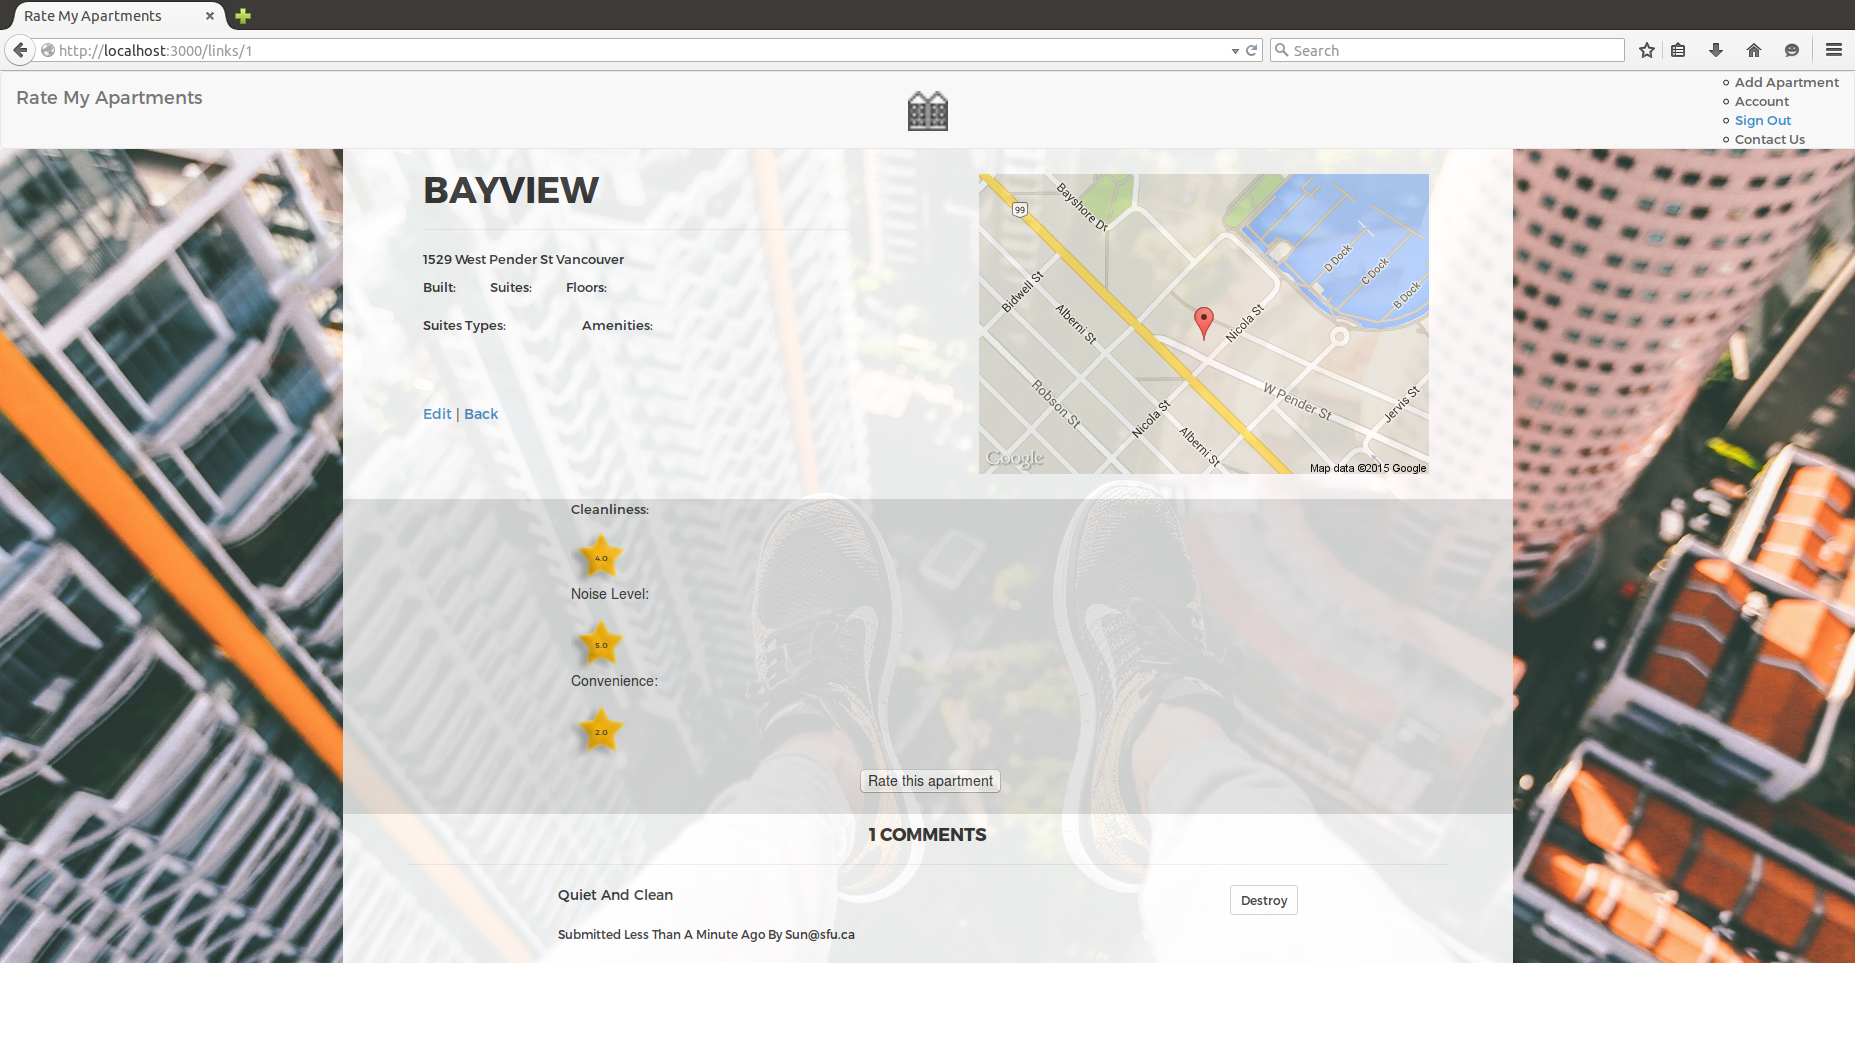
\includegraphics[height=0.5\linewidth]{map.png}
\caption{Map Page}
\end{figure}

\begin{figure}
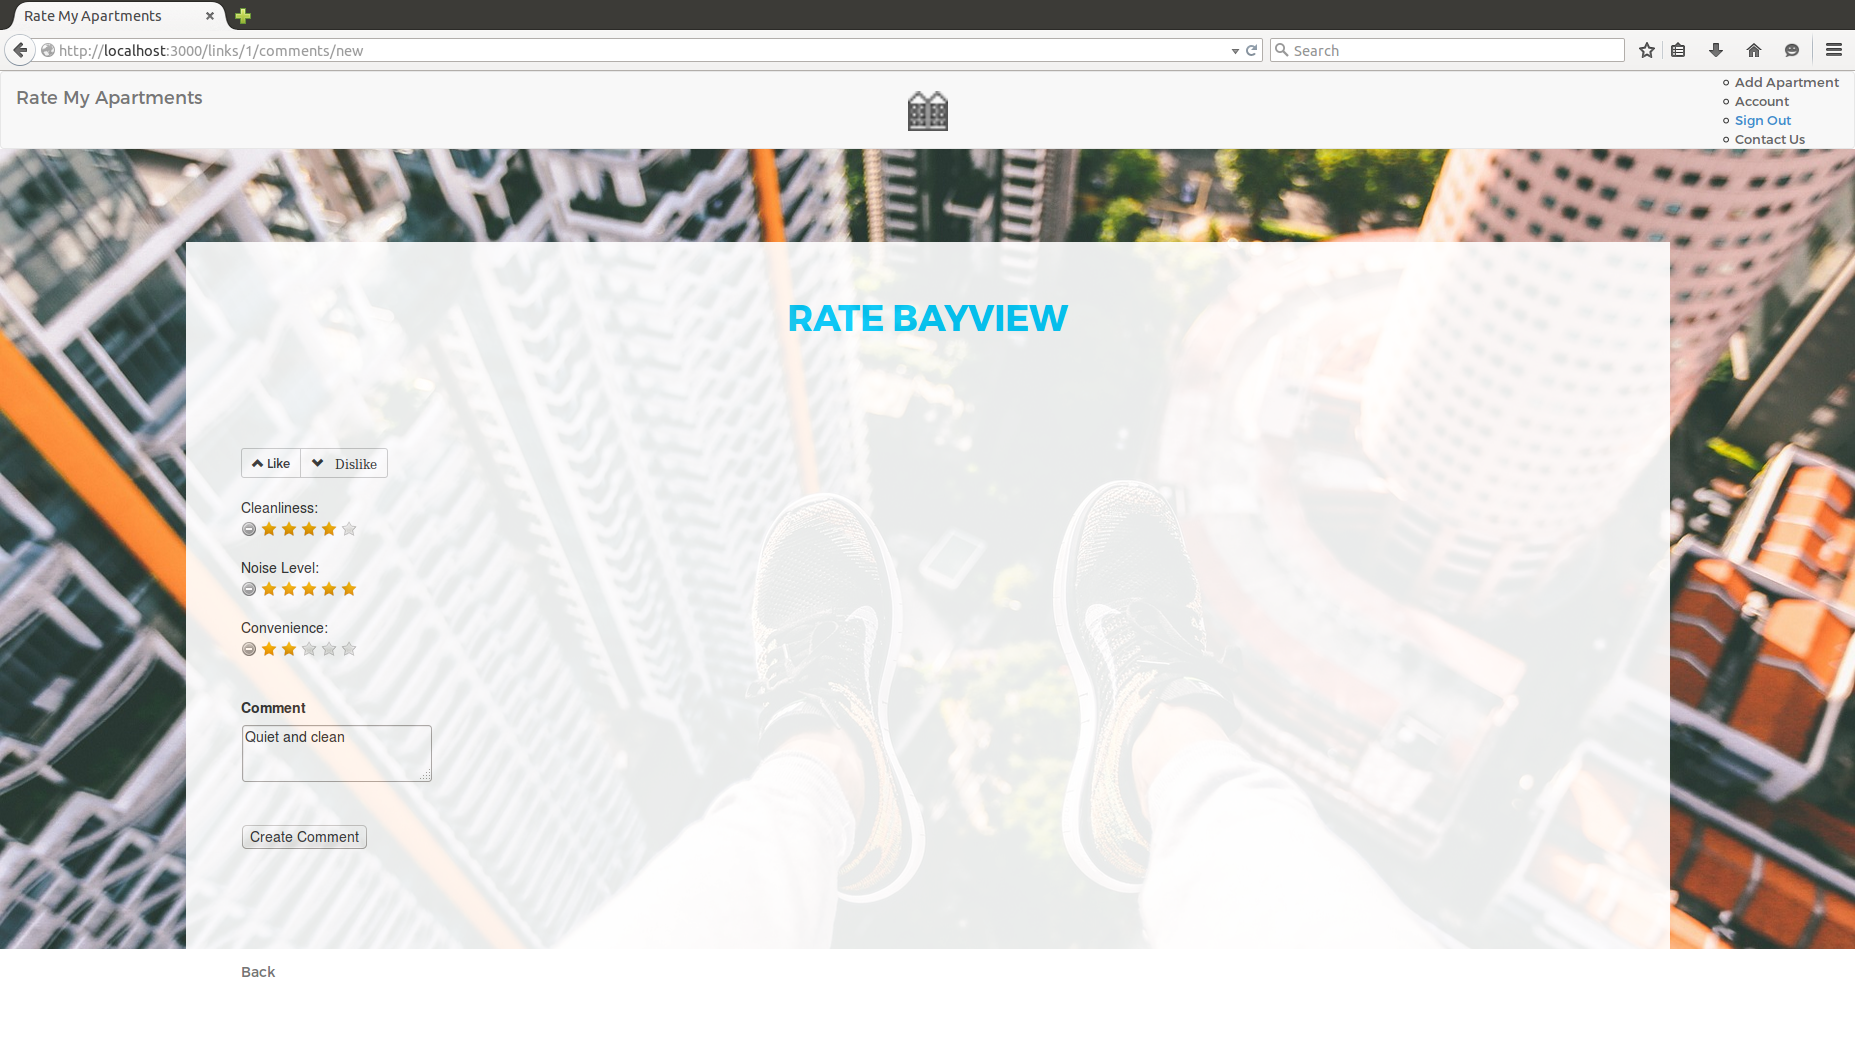
\includegraphics[height=0.5\linewidth]{star.png}
\caption{Star Page}
\end{figure}

%----------------------------------------------------------------------------------------

\end{column} % End of column 2.2

\end{columns} % End of the split of column 2

\end{column} % End of the second column

\begin{column}{\sepwid}\end{column} % Empty spacer column

\begin{column}{\onecolwid} % The third column

%----------------------------------------------------------------------------------------
%	Main function
%----------------------------------------------------------------------------------------
\setbeamercolor{block title}{fg=red,bg=white} % Change the block title color
\begin{block}{Going into more depth...}
\setbeamercolor{block alerted title}{fg=black,bg=norange} % Change the alert block title colors
\setbeamercolor{block alerted body}{fg=black,bg=white} % Change the alert block body colors


- We developed our application using Ruby on Rails framework \newline
- We have chosen RoR because it uses the MVC model, so it allows us to easily implement CRUD operations\newline
- RoR also has a big open-source community that provides us with gems that help us to easily implement features\newline
\end{block}
\begin{alertblock}{Spec/Gem that we used}
- Spec: Ruby on Rails, HTML/CSS, JavaScript, Apache, Passenger, Postgresql, Bootstrap, Git\newline\newline
- Gem: Devise, OmniAuth, Ransack, Rails-autocomplete, Ratyrate, Geocoder, (simple-form)


\end{alertblock}
\begin{figure}
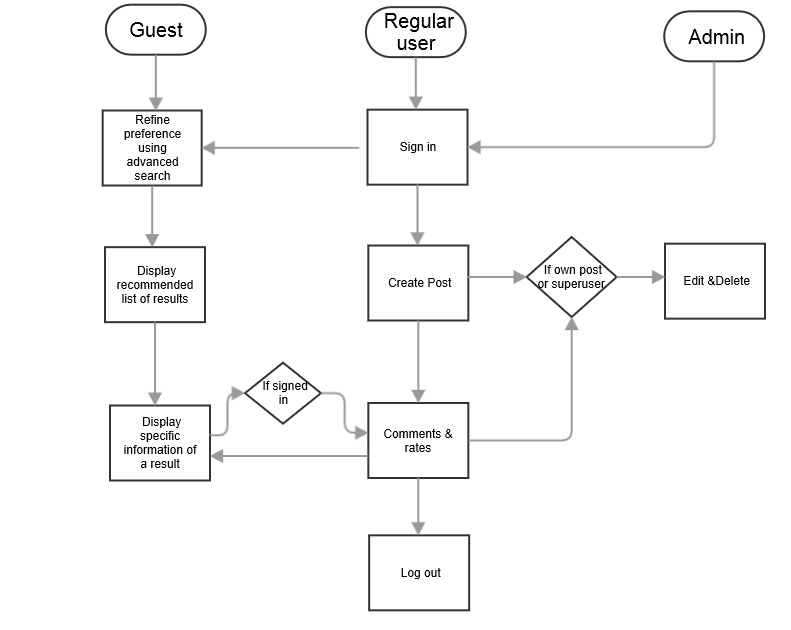
\includegraphics[height=0.6\linewidth]{diagram.png}
\caption{Usecase}
\end{figure}

%----------------------------------------------------------------------------------------
%	CONTACT INFORMATION
%----------------------------------------------------------------------------------------

\setbeamercolor{block alerted title}{fg=black,bg=dorado} % Change the alert block title colors
\setbeamercolor{block alerted body}{fg=black,bg=white} % Change the alert block body colors

\begin{alertblock}{Contact Information}
\begin{itemize}
\item Web: http://cmpt470.csil.sfu.ca:8007
\item Email: cmpt470.mx7@superuser.com
\item Phone: +1 778 822 8882
\end{itemize}
\end{alertblock}
%----------------------------------------------------------------------------------------

\end{column} % End of the third column

\end{columns} % End of all the columns in the poster

\end{frame} % End of the enclosing frame

\end{document}